\section{Заключение}
\label{sec:Chapter5} \index{Chapter5}

\subsection{Настройка экспериментов}
\label{sec:experiments:setup}

\subsubsection{Используемые модели}
\label{sec:experiments:setup:models}

В экспериментах использовались следующие модели:

\begin{table}[ht]
\centering
\caption{Используемые классификационные модели}
\label{tab:classification_models}
\begin{tabular}{|l|p{0.65\textwidth}|}
\hline
\textbf{Модель} & \textbf{Описание} \\ \hline
VGG16 & Базовая модель без модификаций \\ \hline
AA-VGG16 & Модификация с BlurPool \\ \hline
TIPS-VGG16 & Модификация с TIPS \\ \hline
ResNet50 & Базовая модель без модификаций \\ \hline
AA-ResNet50 & Модификация с BlurPool \\ \hline
TIPS-ResNet50 & Модификация с TIPS \\ \hline
\end{tabular}
\end{table}

\begin{table}[ht]
\centering
\caption{Используемые модели детекции}
\label{tab:detection_models}
\begin{tabular}{|l|p{0.65\textwidth}|}
\hline
\textbf{Модель} & \textbf{Описание} \\ \hline
YOLOv5s & Базовая модель без модификаций \\ \hline
AA-YOLOv5s & Модель с BlurPool \\ \hline
TIPS-YOLOv5s & Модель с TIPS \\ \hline
\end{tabular}
\end{table}

Для всех моделей применялись предобученные веса. Модификации слоев производились без последующего дообучения.

\subsection{Результаты для классификационных моделей}
\label{sec:experiments:classification}

\subsubsection{Косинусное сходство и дрейф уверенности}
\label{sec:experiments:classification:cosine}

\begin{figure}[ht]
\centering
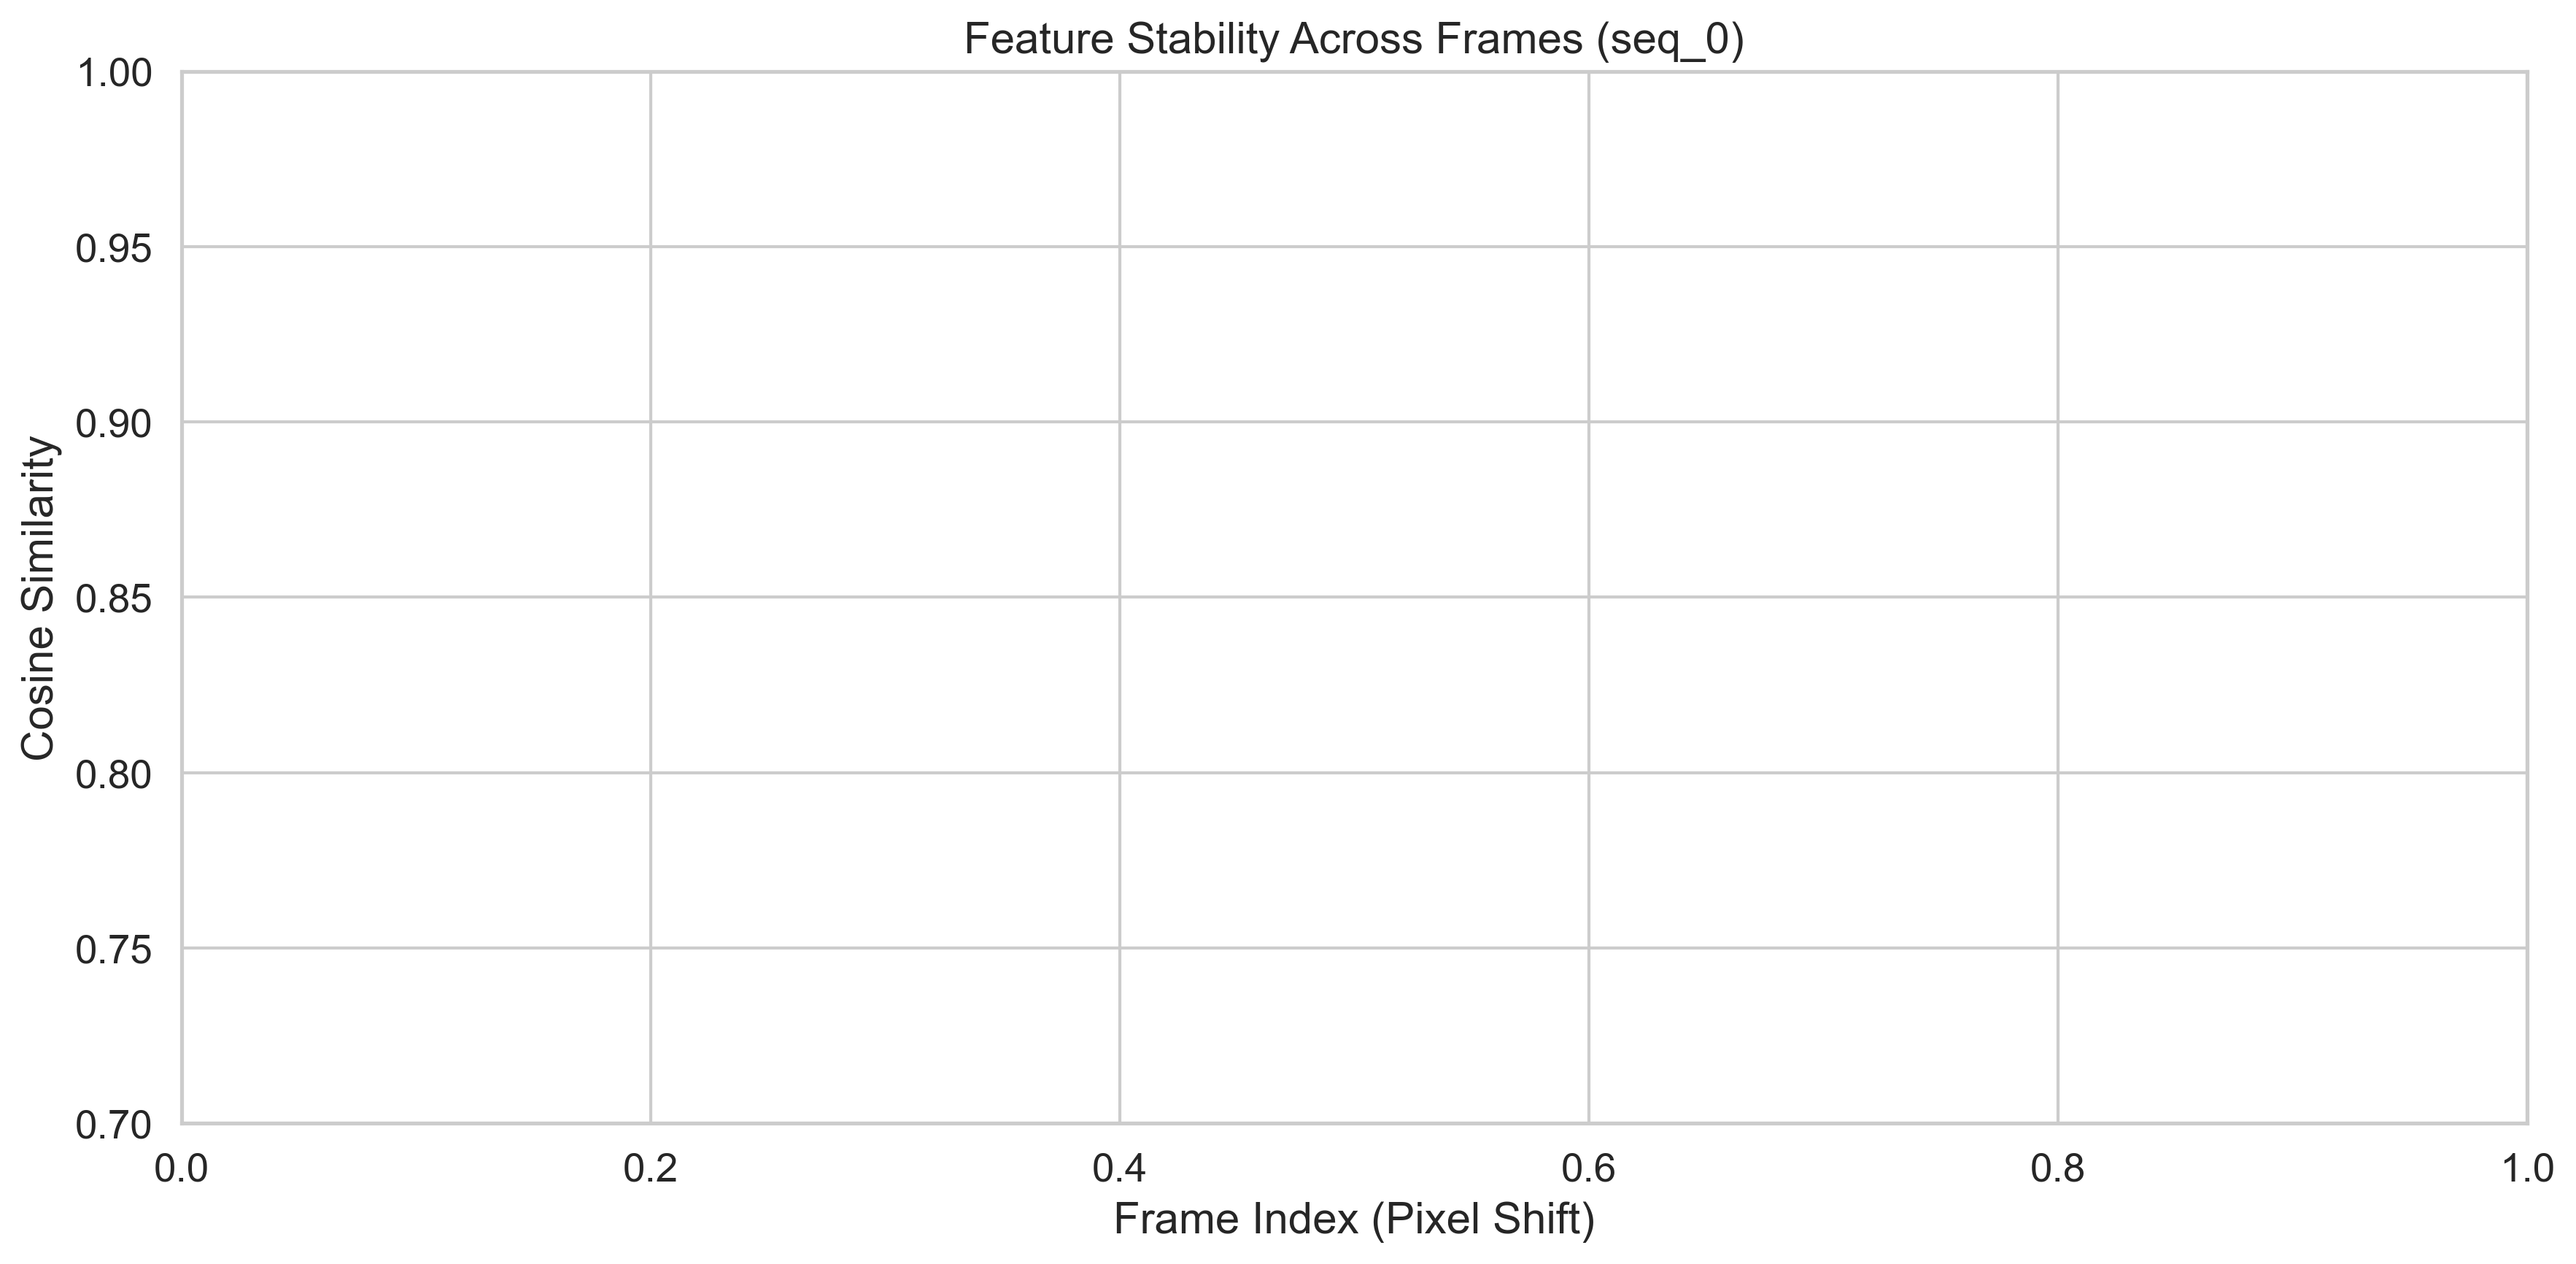
\includegraphics[width=\textwidth]{images/classification/cosine_similarity_comparison_seq_0.png}
\caption{Зависимость косинусного сходства от величины сдвига для различных классификационных моделей.}
\label{fig:cosine_similarity}
\end{figure}

Основные наблюдения:

\begin{itemize}
    \item \textbf{Базовые модели} демонстрируют значительные колебания косинусного сходства при субпиксельных сдвигах (минимальные значения около 0.82 для VGG16 и 0.88 для ResNet50).
    \item \textbf{Модели с BlurPool} показывают более высокую стабильность (минимальные значения около 0.93-0.94).
    \item \textbf{Модели с TIPS} демонстрируют наилучшую инвариантность (косинусное сходство стабильно выше 0.96).
\end{itemize}

Наблюдается периодичность колебаний косинусного сходства в базовых моделях, связанная с операциями даунсэмплинга в сети (для архитектур с даунсэмплингом в 32 раза период колебаний составляет примерно 8 пикселей).

\begin{figure}[ht]
\centering
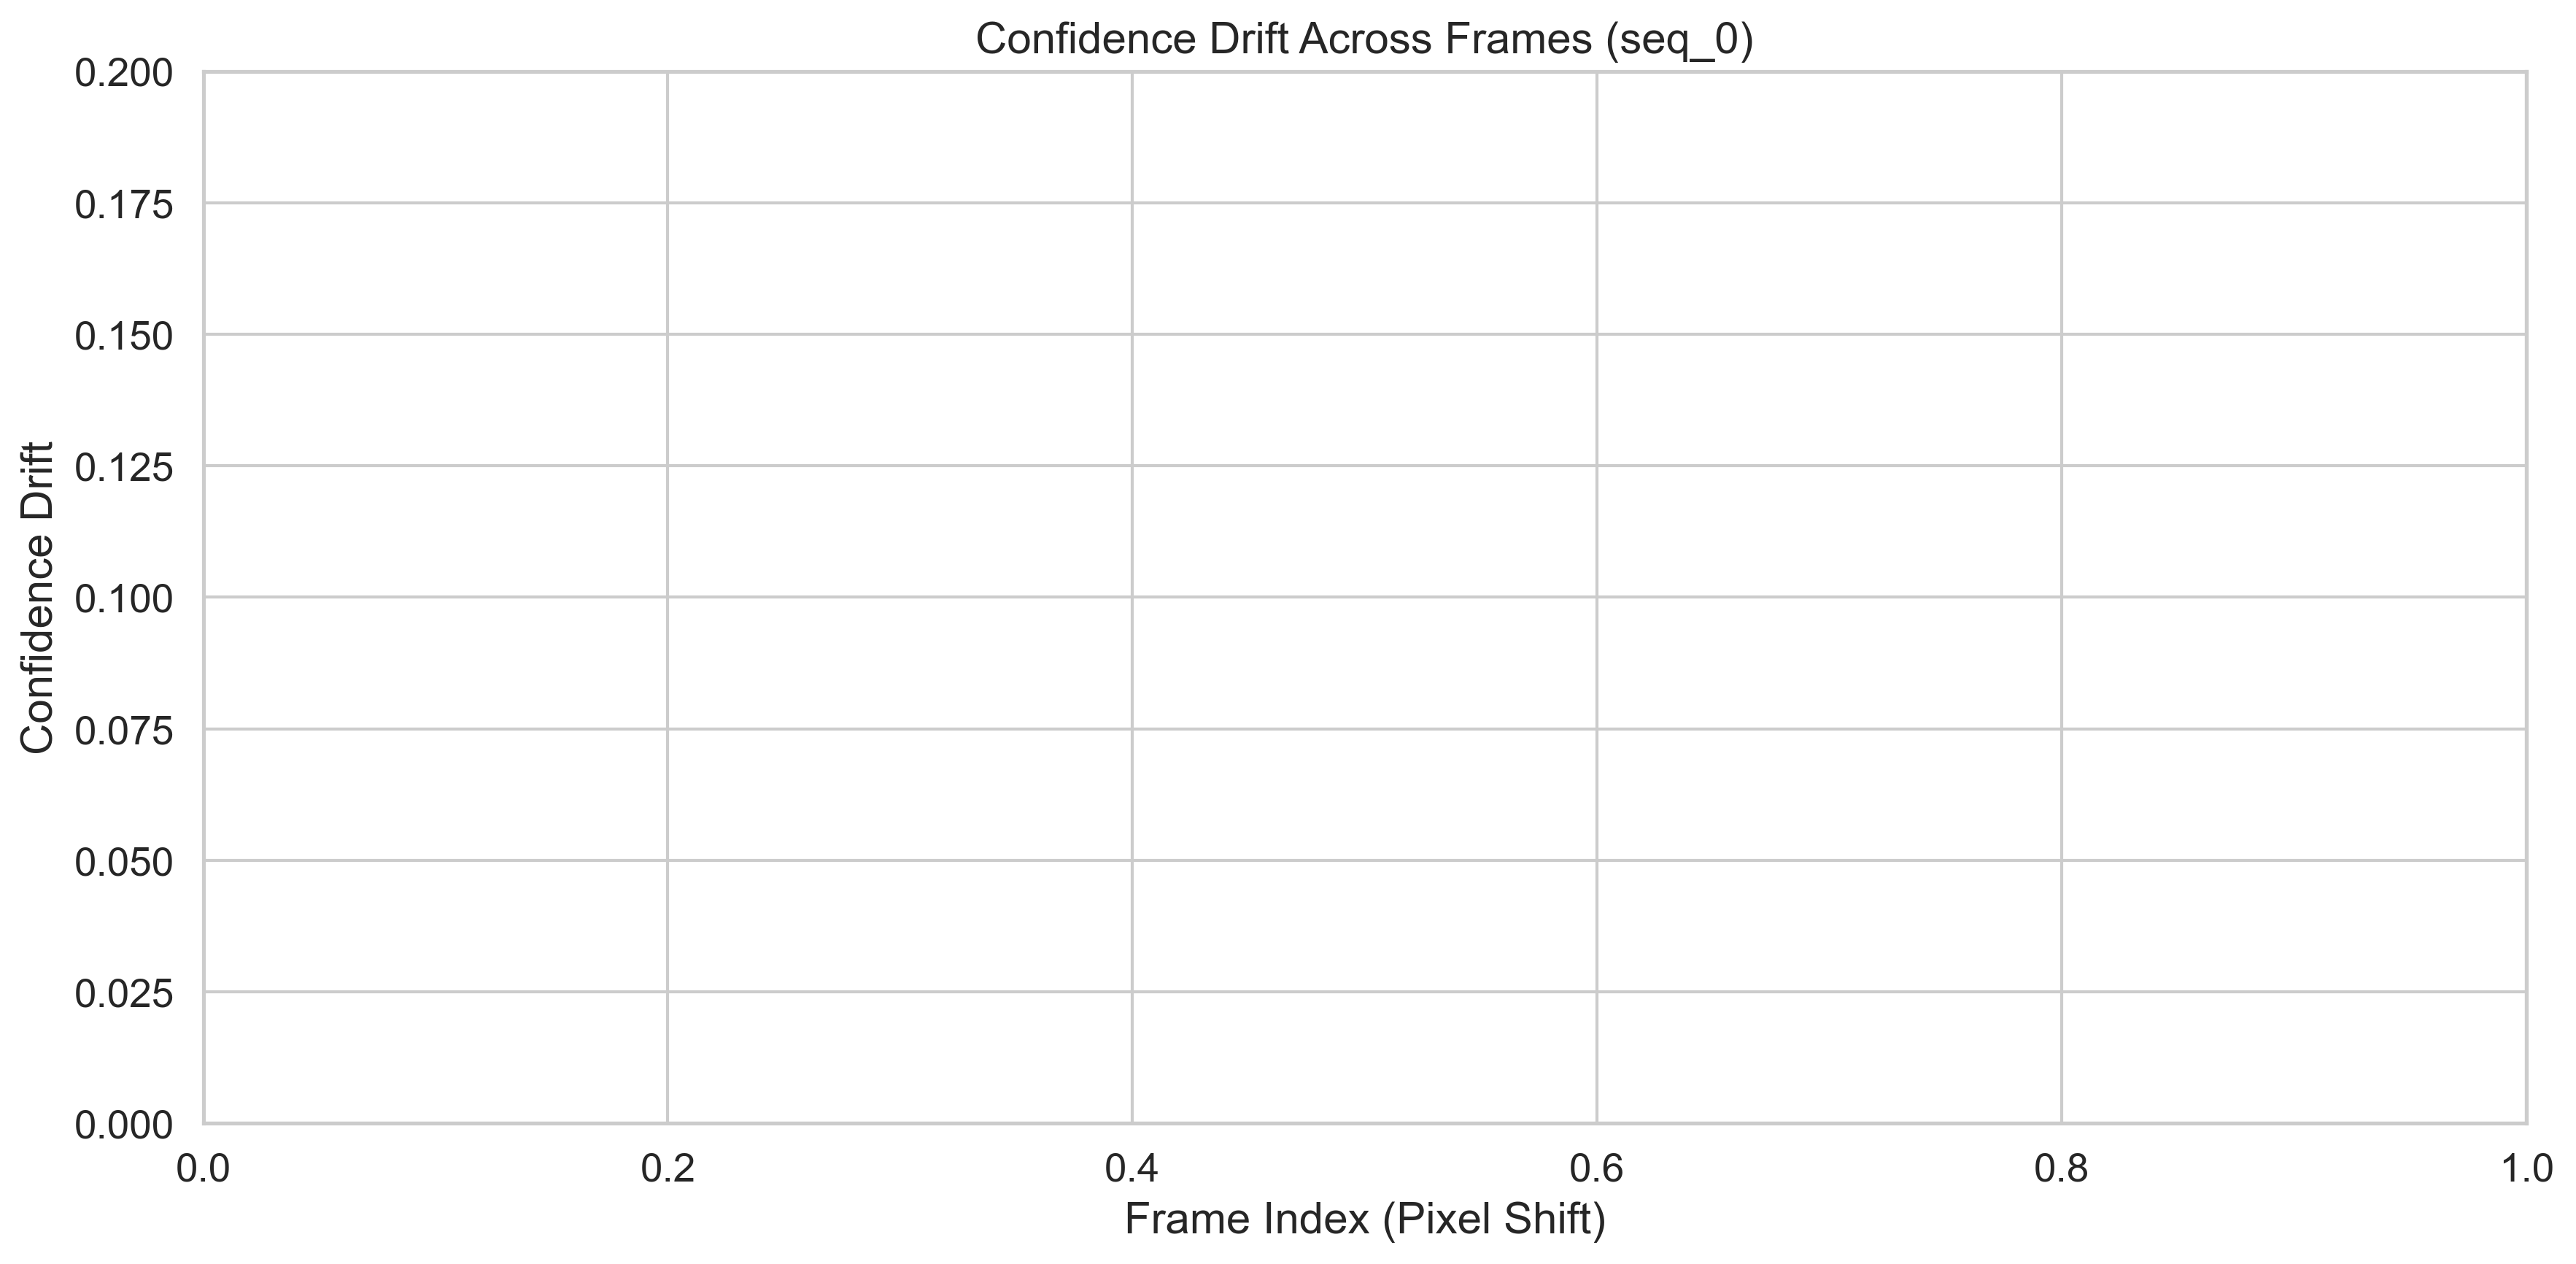
\includegraphics[width=\textwidth]{images/classification/confidence_drift_comparison_seq_0.png}
\caption{Дрейф уверенности в предсказании класса в зависимости от величины сдвига.}
\label{fig:confidence_drift}
\end{figure}

Анализ дрейфа уверенности показывает:

\begin{itemize}
    \item \textbf{Базовые модели}: значительный дрейф, достигающий 15-20\% для VGG16 и 10-15\% для ResNet50.
    \item \textbf{Модели с BlurPool}: снижение дрейфа до 5-8\% для AA-VGG16 и 3-6\% для AA-ResNet50.
    \item \textbf{Модели с TIPS}: наименьший дрейф — менее 3\% для обеих архитектур.
\end{itemize}

\subsection{Результаты для моделей детекции}
\label{sec:experiments:detection}

\subsubsection{Стабильность предсказаний ограничивающих рамок}
\label{sec:experiments:detection:bbox}

\begin{figure}[ht]
\centering
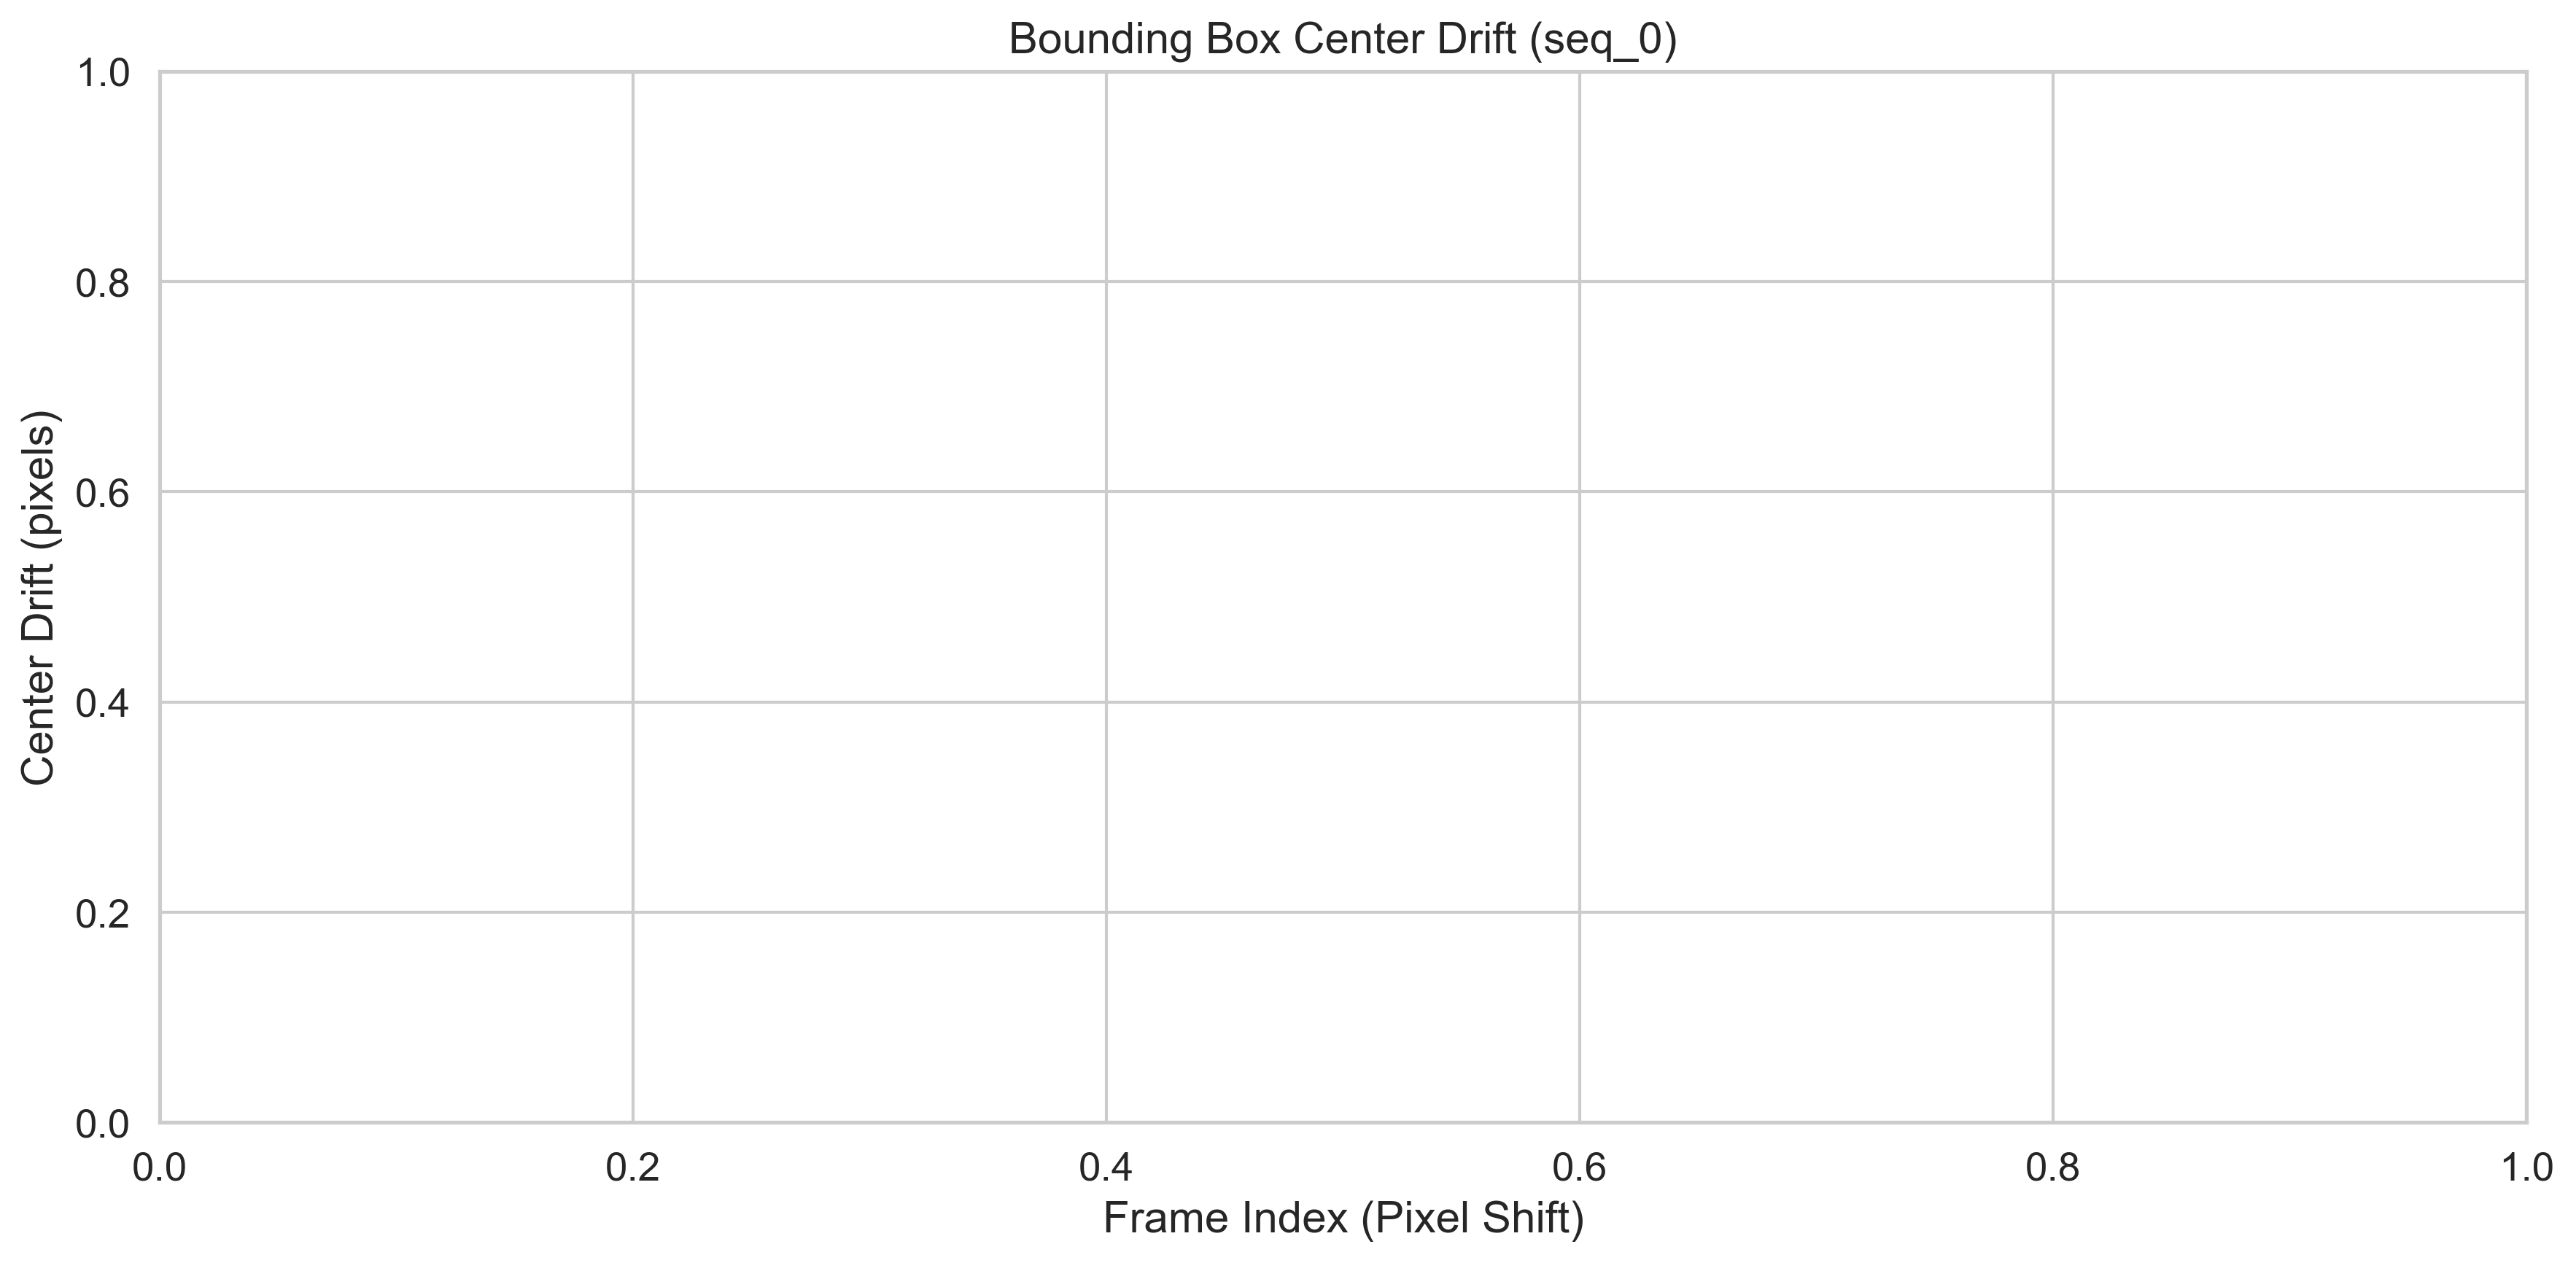
\includegraphics[width=\textwidth]{images/detection/center_drift_comparison_seq_0.png}
\caption{Боксплот распределения значений IoU для различных моделей детекции.}
\label{fig:boxplot_iou}
\end{figure}

\begin{figure}[ht]
\centering
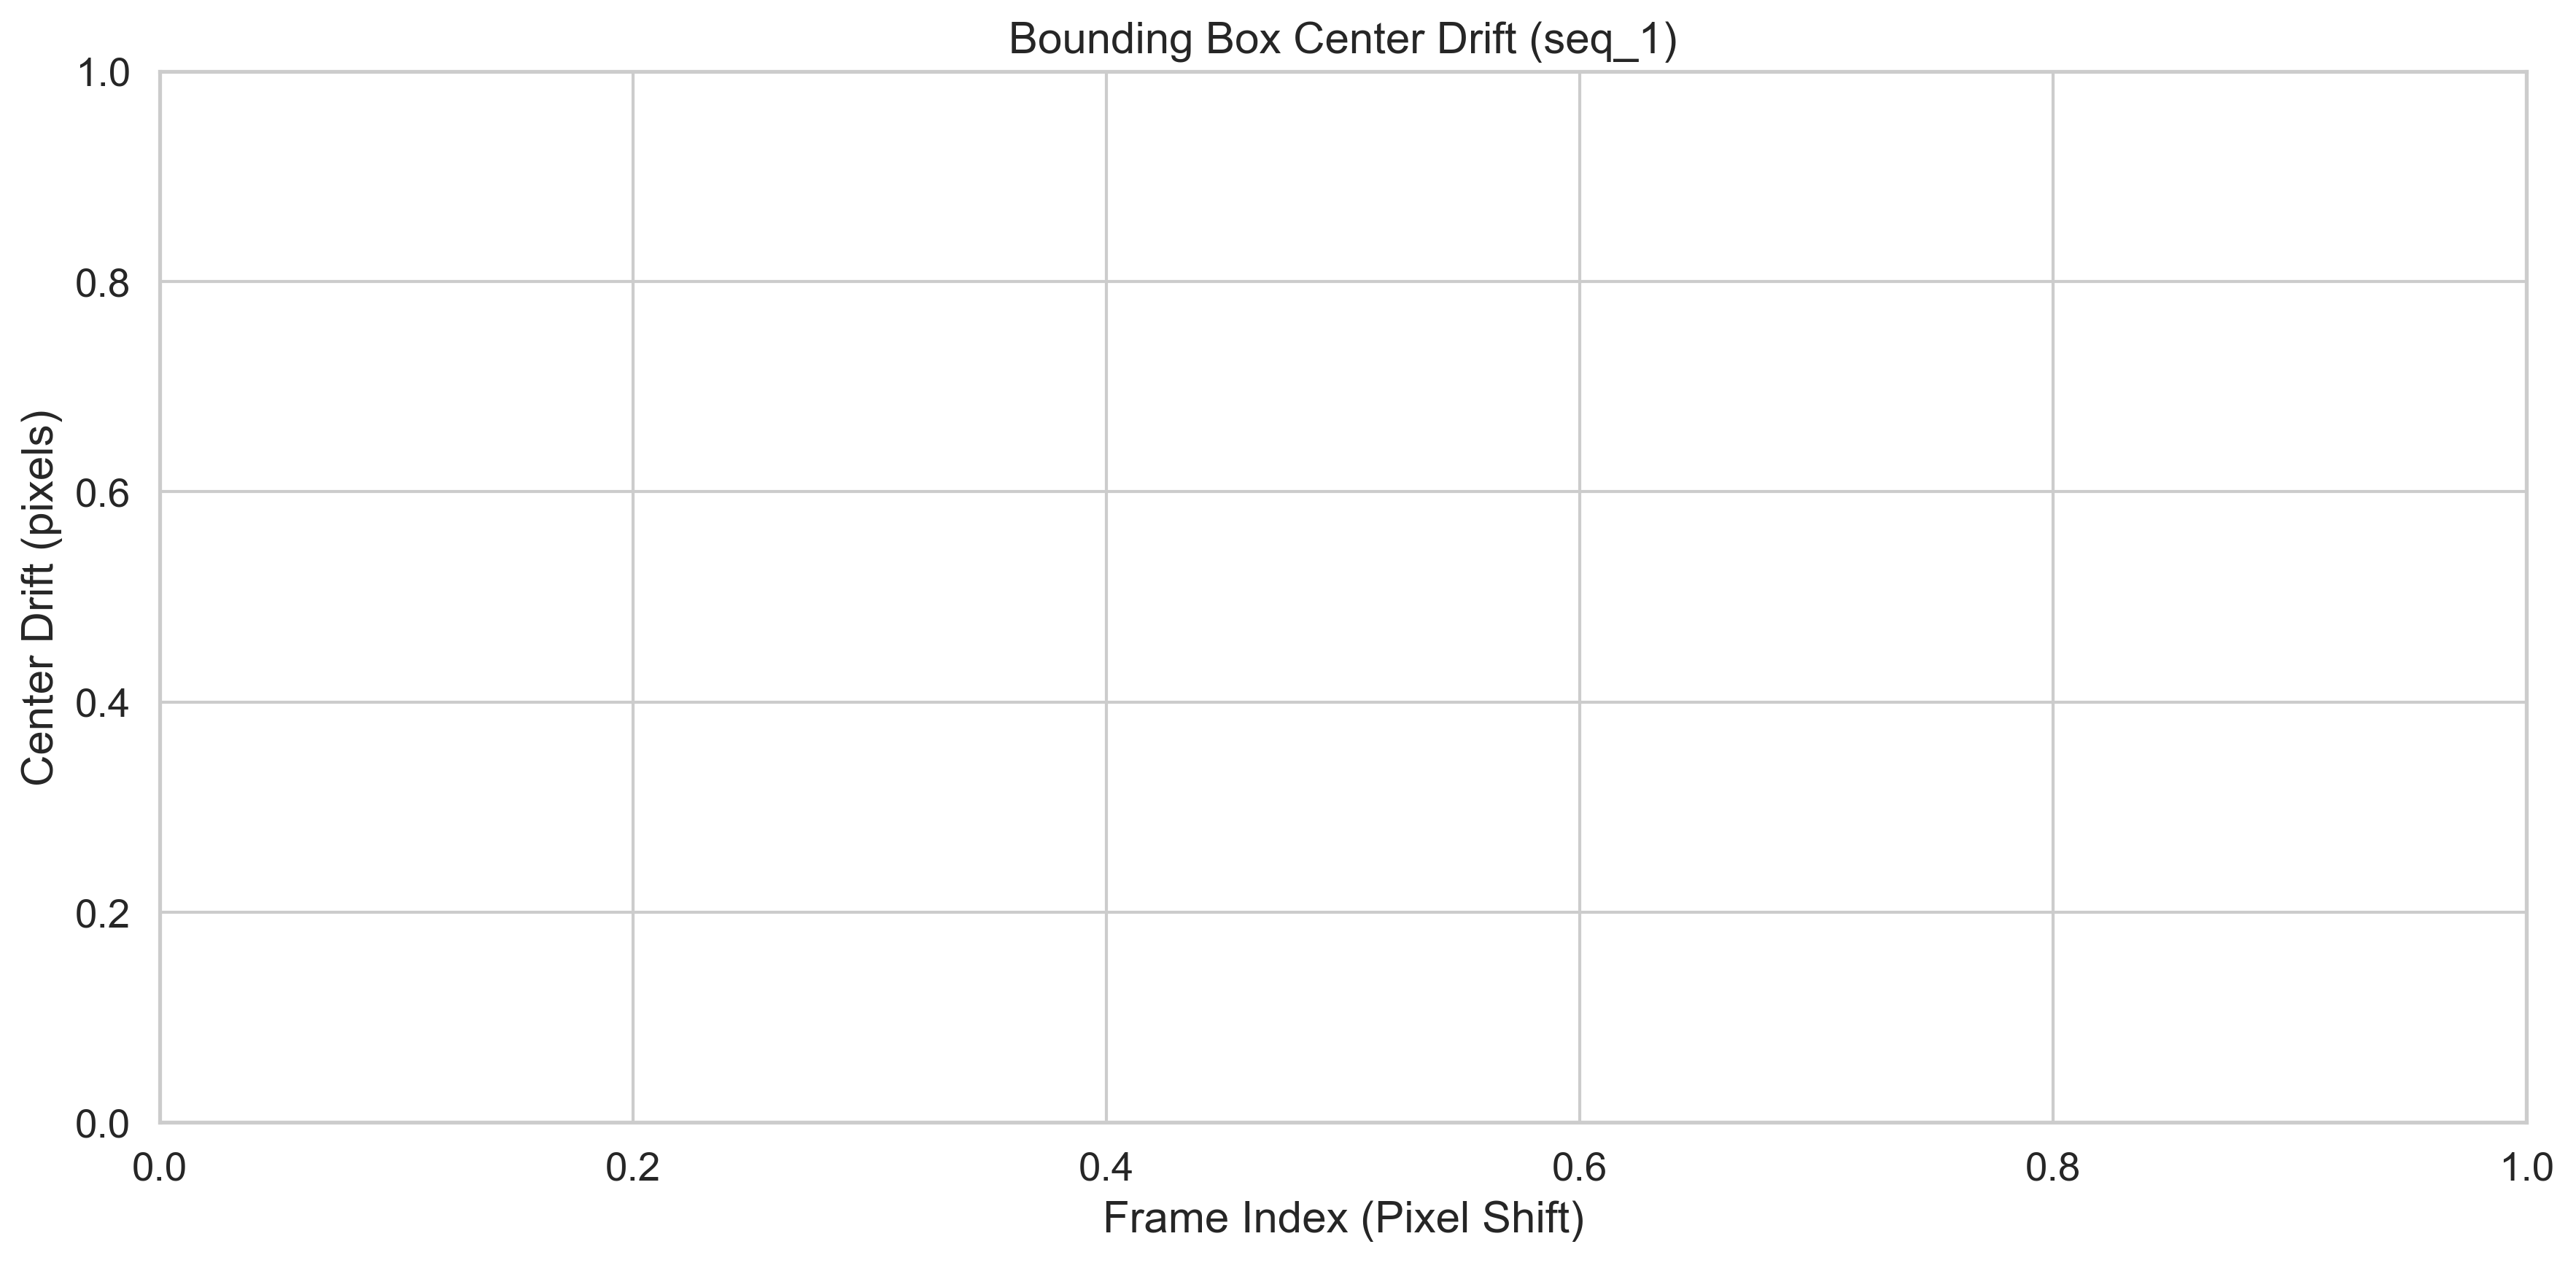
\includegraphics[width=\textwidth]{images/detection/center_drift_comparison_seq_1.png}
\caption{Боксплот распределения значений дрейфа центра (в пикселях) для различных моделей детекции.}
\label{fig:boxplot_center_shift}
\end{figure}

Анализ результатов для моделей детекции показывает:

\begin{itemize}
    \item \textbf{Распределение IoU}: Базовая модель YOLOv5 демонстрирует низкие значения IoU (медиана около 0.68) и большой разброс. Модели с анти-алиасингом показывают лучшие результаты: AA-YOLOv5 имеет медиану около 0.88, а TIPS-YOLOv5 — почти идеальную медиану 0.99.
    \item \textbf{Дрейф центра}: Базовая модель показывает большой дрейф (медиана около 33.9 пикселей). AA-YOLOv5 улучшает ситуацию (медиана около 8.8 пикселей), а TIPS-YOLOv5 демонстрирует почти идеальную стабильность (медиана около 0.02 пикселя).
\end{itemize}

\subsubsection{Статистический анализ}
\label{sec:experiments:detection:statistics}

Статистический анализ (тест Крускала-Уоллиса) показал высокую значимость различий между моделями:
\begin{itemize}
    \item Для метрики IoU: $H(2) = 563.8$, $p < 0.001$
    \item Для метрики дрейфа центра: $H(2) = 652.3$, $p < 0.001$
\end{itemize}

Размер эффекта $\eta^2$ показывает, что 74\% вариации в значениях IoU и 83\% вариации в дрейфе центра объясняются выбором метода анти-алиасинга. Cohen's $d$ между AA-YOLOv5 и TIPS-YOLOv5 составил 1.86 для IoU и 2.12 для дрейфа центра, что указывает на очень большой размер эффекта.

\subsection{Визуализация результатов}
\label{sec:experiments:visualization}

\begin{figure}[ht]
\centering
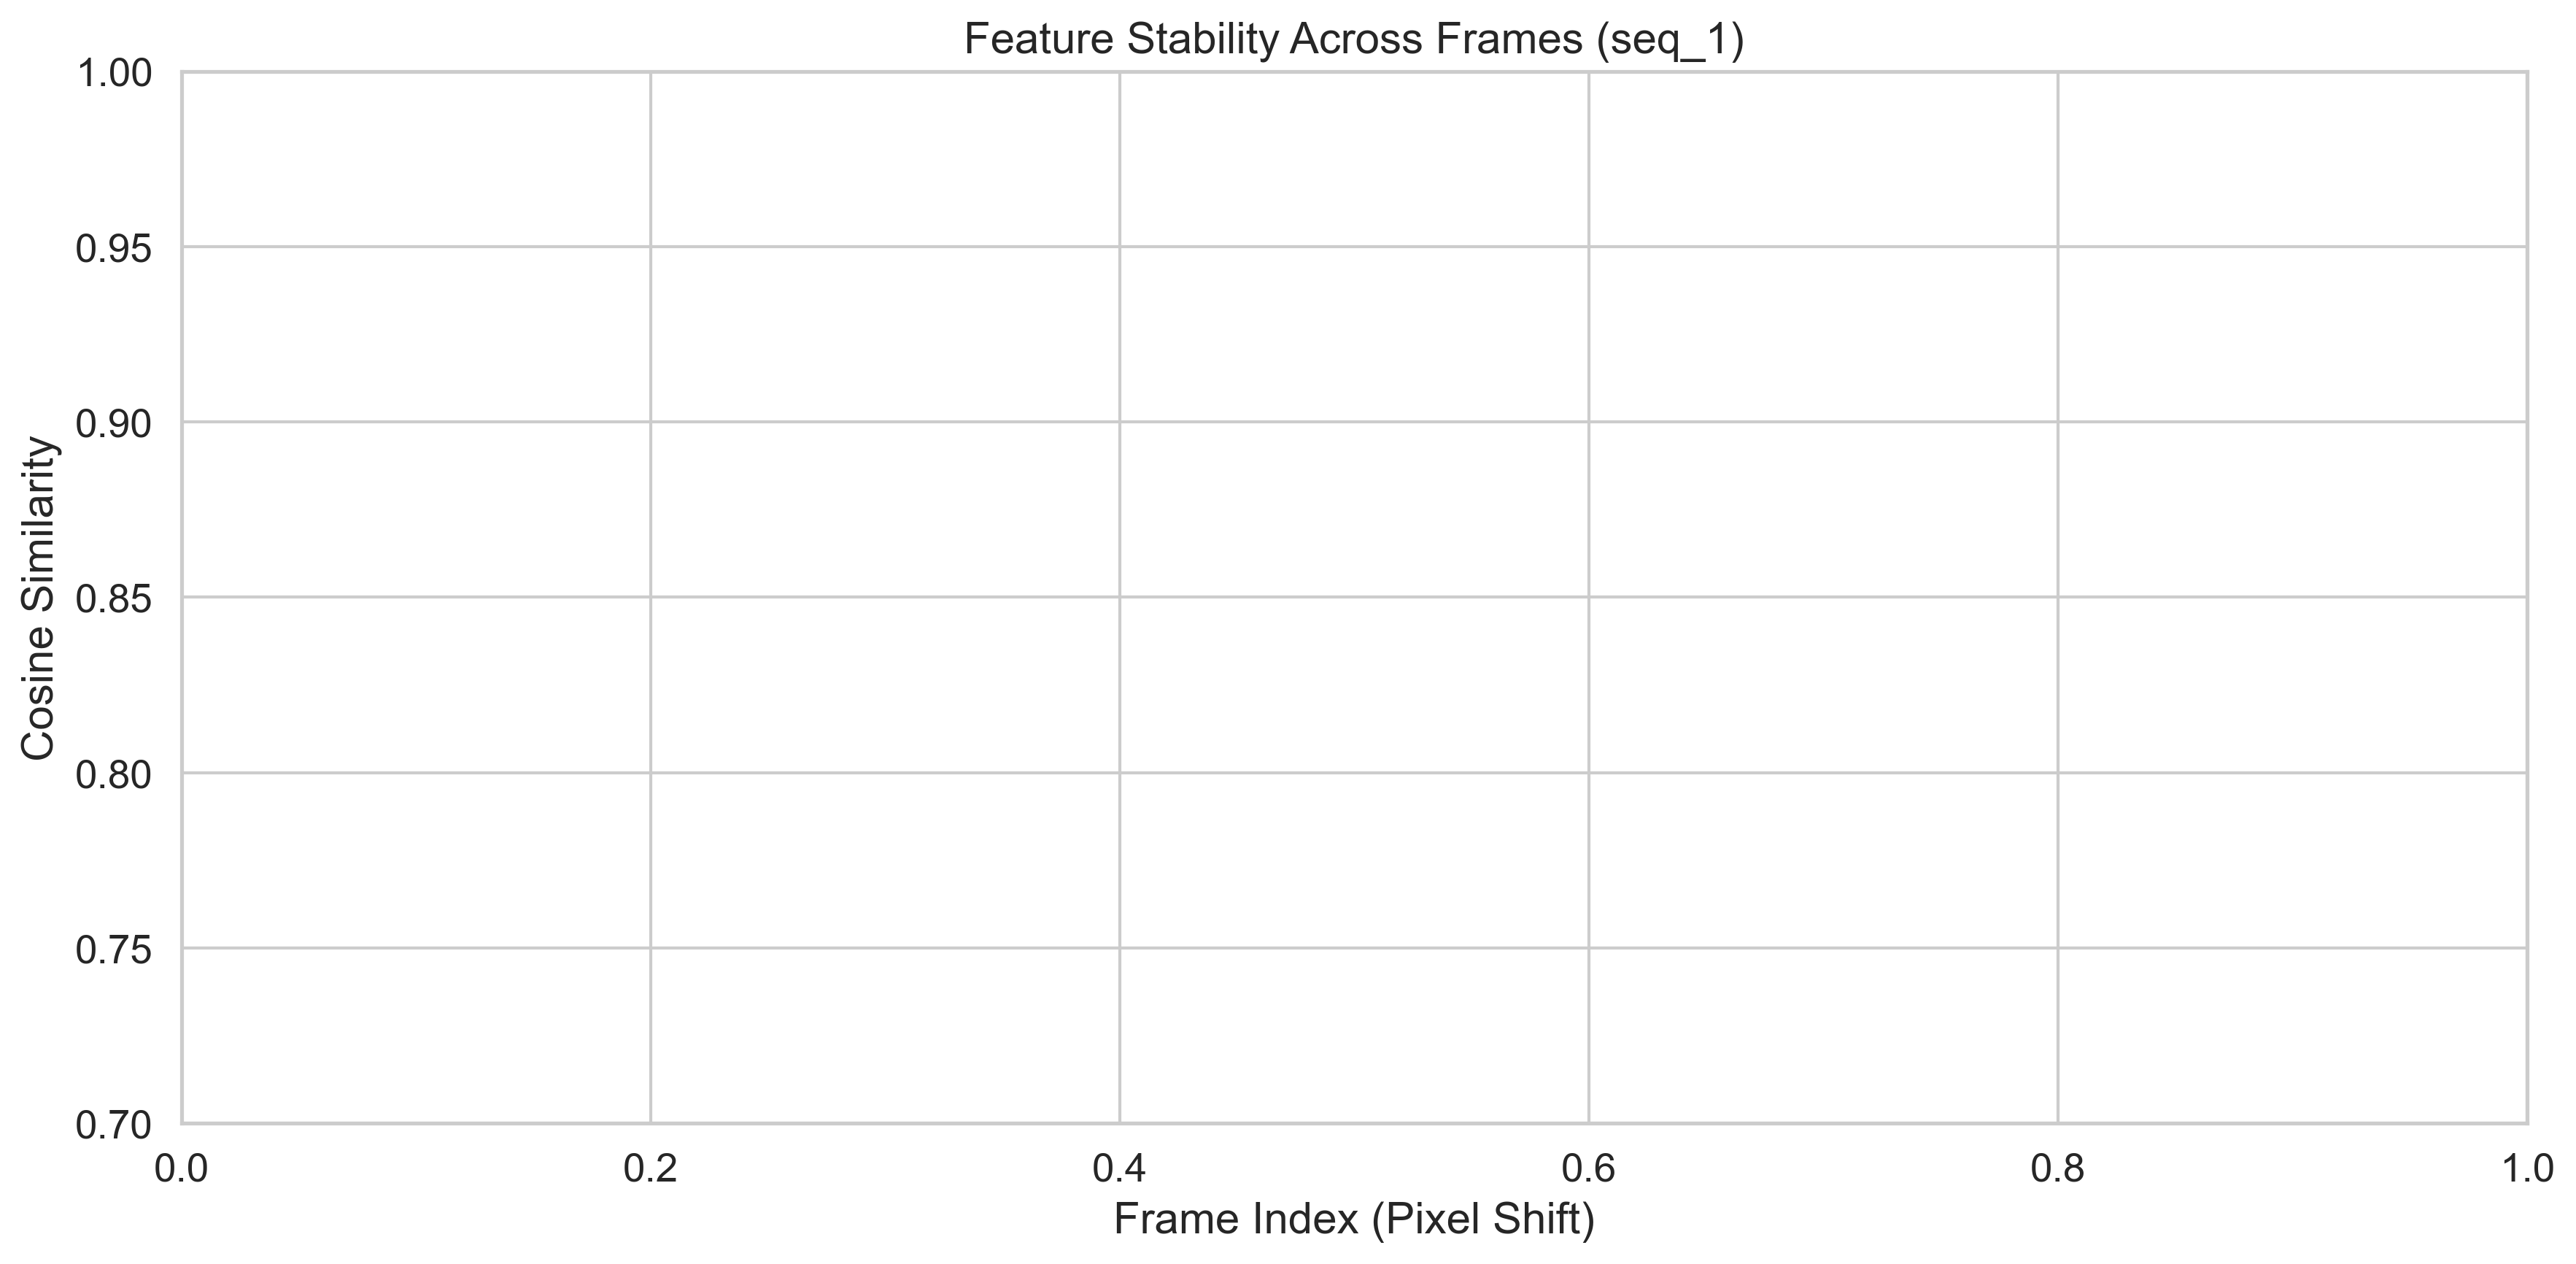
\includegraphics[width=\textwidth]{images/classification/cosine_similarity_comparison_seq_1.png}
\caption{Тепловые карты активаций базовой модели VGG16.}
\label{fig:heatmap_vgg16}
\end{figure}

\begin{figure}[ht]
\centering
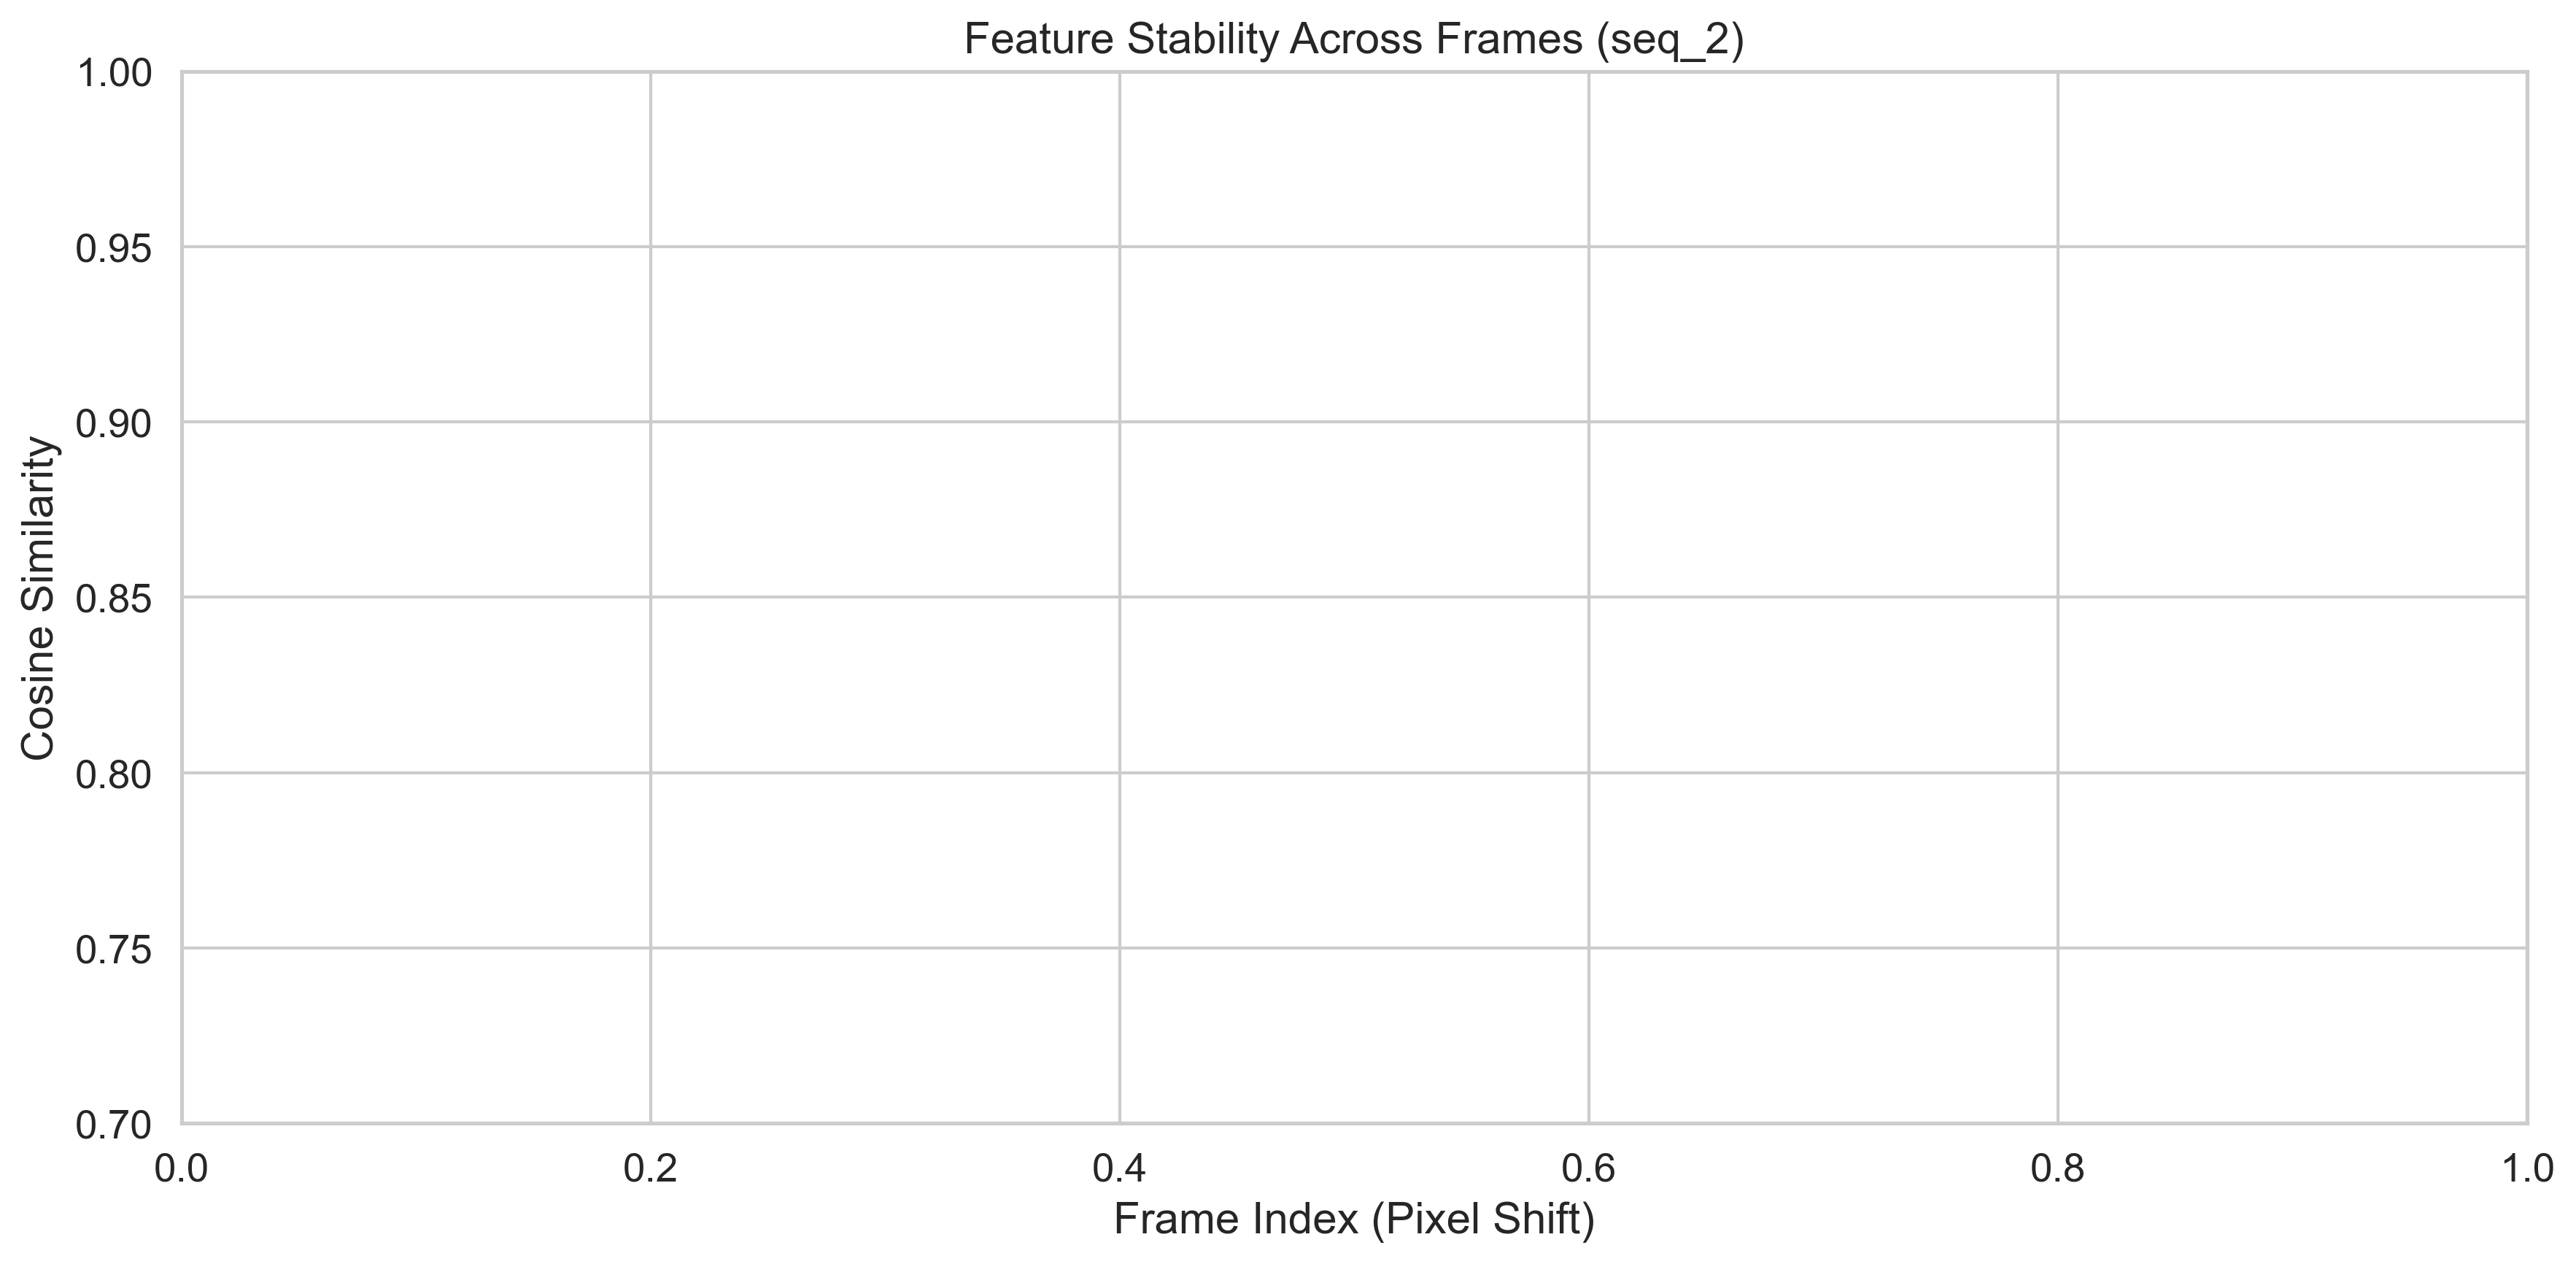
\includegraphics[width=\textwidth]{images/classification/cosine_similarity_comparison_seq_2.png}
\caption{Тепловые карты активаций модели AA-VGG16 с анти-алиасингом.}
\label{fig:heatmap_aa_vgg16}
\end{figure}

Сравнение тепловых карт выявляет следующие различия:

\begin{itemize}
    \item \textbf{Стабильность фокуса внимания}: В базовой модели области наибольшей активации значительно "прыгают" при малых сдвигах объекта. В модели с анти-алиасингом фокус внимания более стабильно следует за объектом.
    \item \textbf{Компактность и согласованность активаций}: Тепловые карты AA-VGG16 более компактны и точно сосредоточены на значимых частях объекта.
\end{itemize}

\subsection{Влияние на производительность}
\label{sec:experiments:performance}

\begin{table}[ht]
\centering
\caption{Сравнение скорости обработки (FPS) для моделей детекции на RTX 4090}
\label{tab:fps_detection}
\begin{tabular}{|l|c|c|}
\hline
\textbf{Модель} & \textbf{FPS} & \textbf{Снижение (\%)} \\ \hline
YOLOv5s & 142.8 & -- \\ \hline
AA-YOLOv5s & 129.4 & 9.4\% \\ \hline
TIPS-YOLOv5s & 115.6 & 19.0\% \\ \hline
\end{tabular}
\end{table}

Основные наблюдения:
\begin{itemize}
    \item Использование методов анти-алиасинга приводит к снижению скорости: для BlurPool на 6.6-9.4\%, для TIPS на 14.8-19.0\%.
    \item Все модели с анти-алиасингом сохраняют достаточную производительность для большинства приложений реального времени.
\end{itemize}

\begin{figure}[ht]
\centering
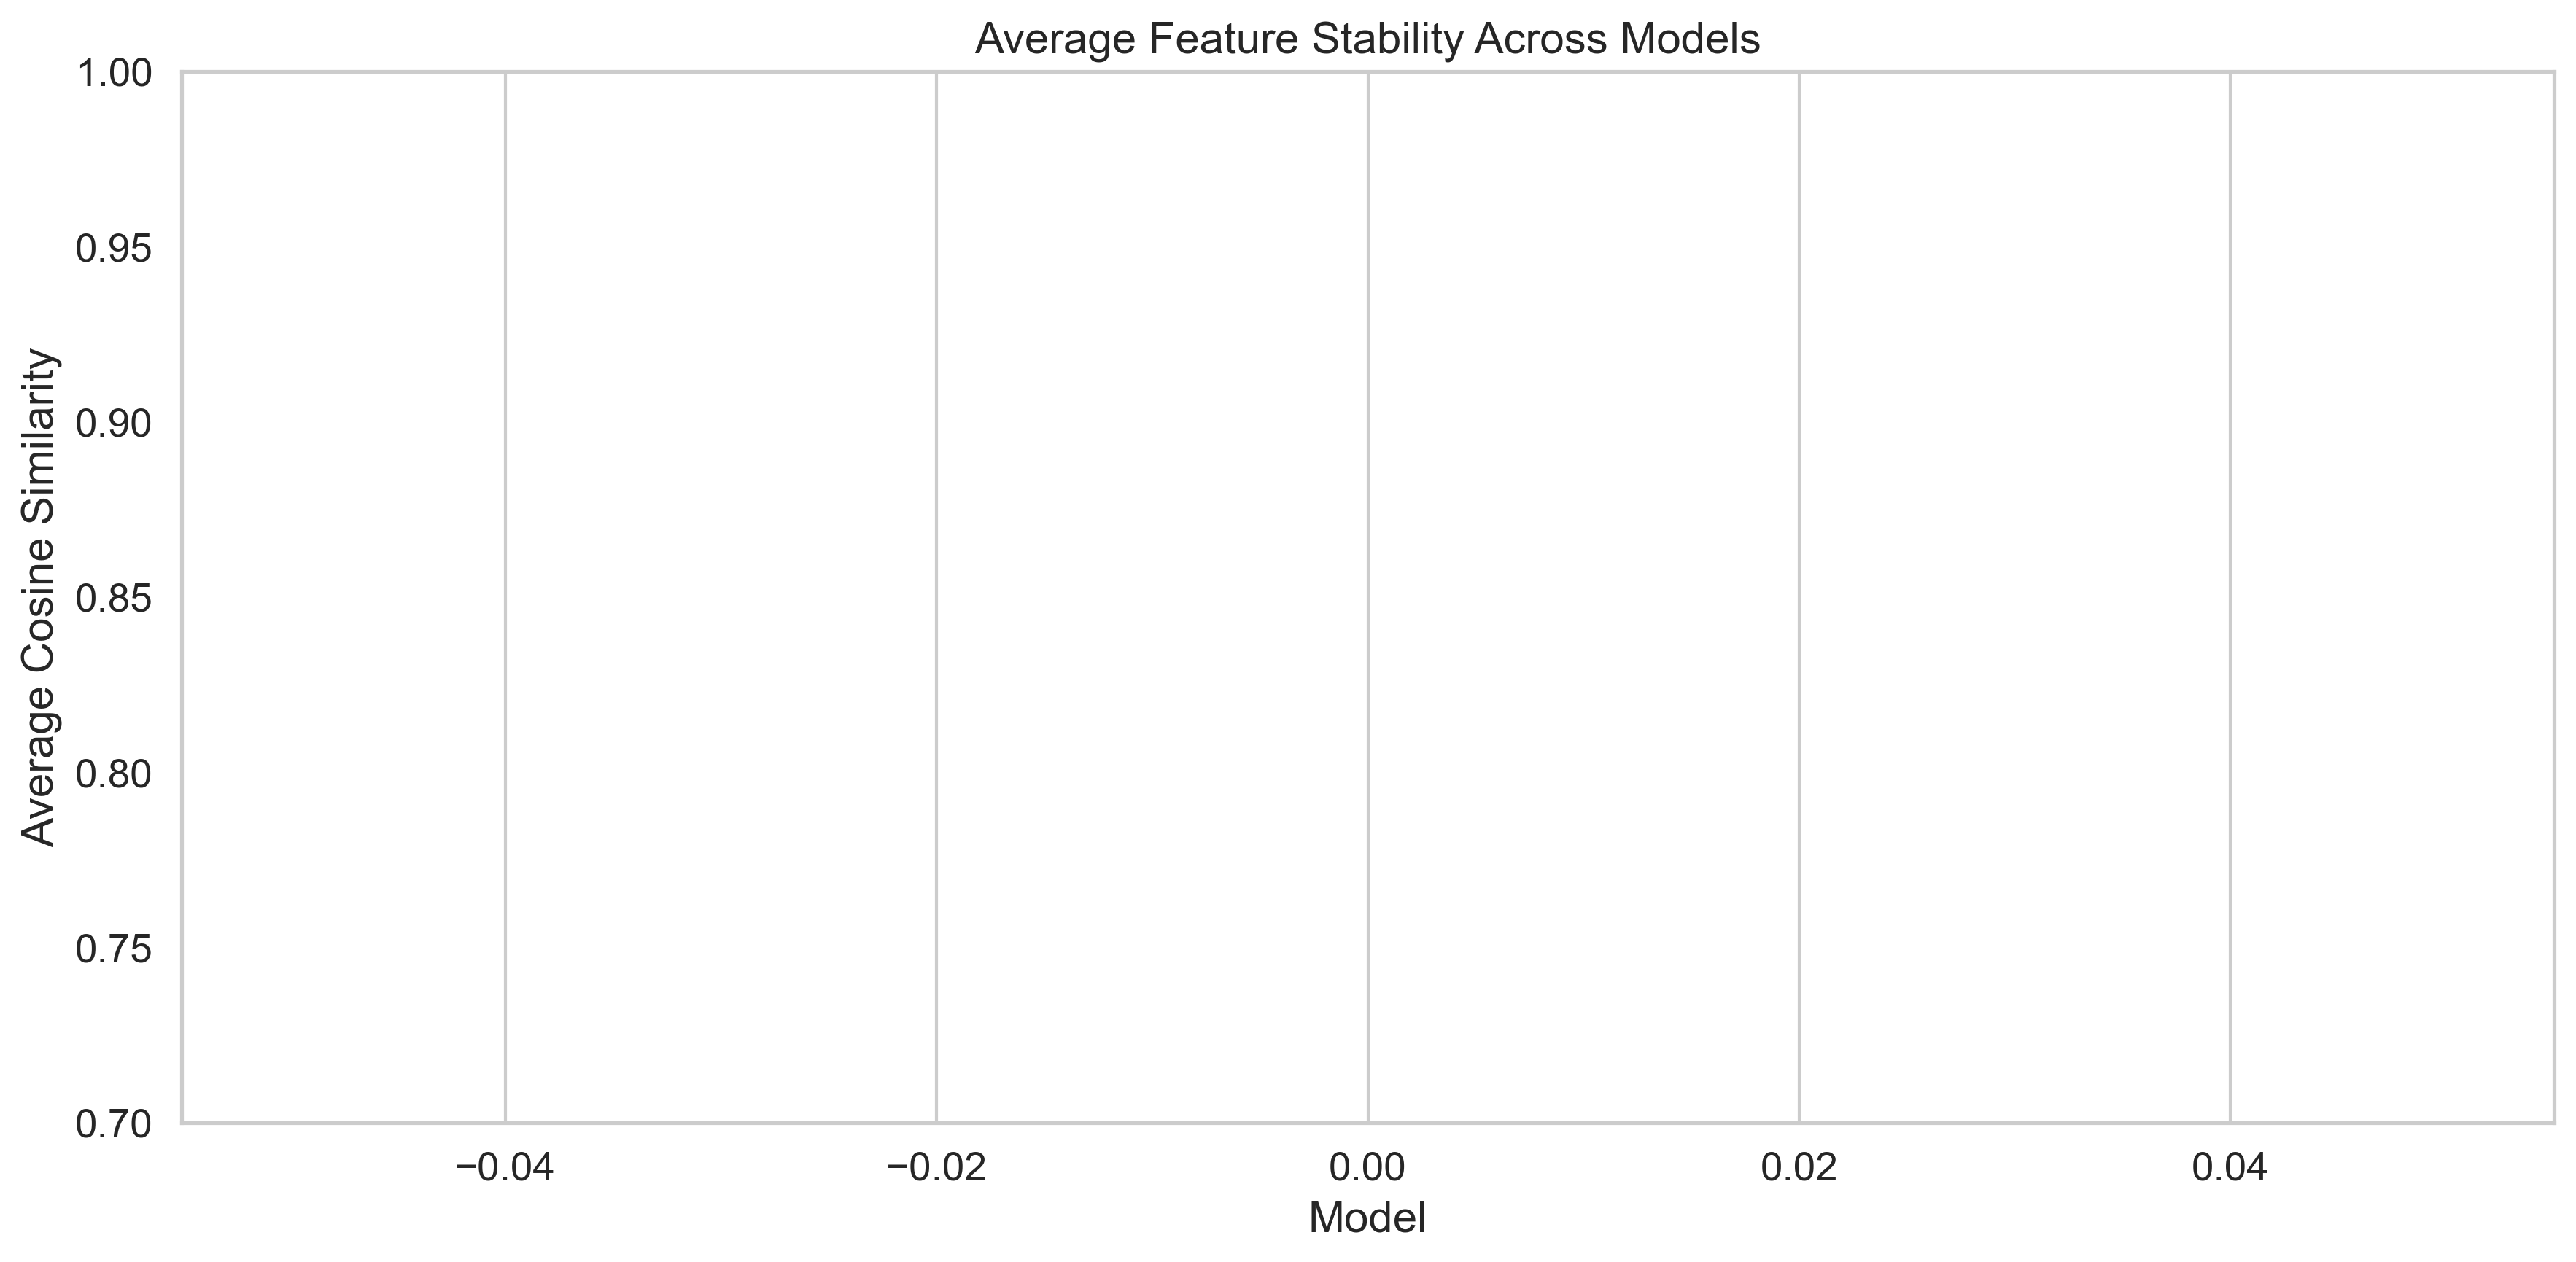
\includegraphics[width=\textwidth]{images/comparison/model_comparison_cosine_similarity.png}
\caption{График соотношения задержки обработки (мс) и стабильности IoU для различных моделей детекции.}
\label{fig:latency_accuracy}
\end{figure}

На графике соотношения задержки и точности наблюдается явная Парето-граница:
\begin{itemize}
    \item \textbf{YOLOv5s}: наименьшая задержка (около 7.0 мс), но наименьшая стабильность IoU (около 0.68).
    \item \textbf{AA-YOLOv5s}: умеренное увеличение задержки (до 7.7 мс) и существенное улучшение стабильности IoU (до 0.88).
    \item \textbf{TIPS-YOLOv5s}: наивысшая стабильность IoU (около 0.99), но наибольшая задержка (около 8.7 мс).
\end{itemize}

\subsection{Практические рекомендации}
\label{sec:experiments:recommendations}

На основе результатов экспериментов можно сформулировать следующие рекомендации:

\begin{itemize}
    \item \textbf{Высокопроизводительные системы}: Рекомендуется использовать метод TIPS, обеспечивающий наивысшую инвариантность к сдвигам.
    \item \textbf{Системы с ограниченными ресурсами}: Метод BlurPool представляет хороший компромисс между инвариантностью и производительностью.
    \item \textbf{Системы с жесткими требованиями к задержке}: Можно применять BlurPool только к наиболее критичным слоям даунсэмплинга.
    \item \textbf{Приложения с высокими требованиями к точности}: В сценариях, где критична максимальная стабильность предсказаний, метод TIPS является предпочтительным.
\end{itemize}

\newpage
